
\begin{figure*}
	\centering
	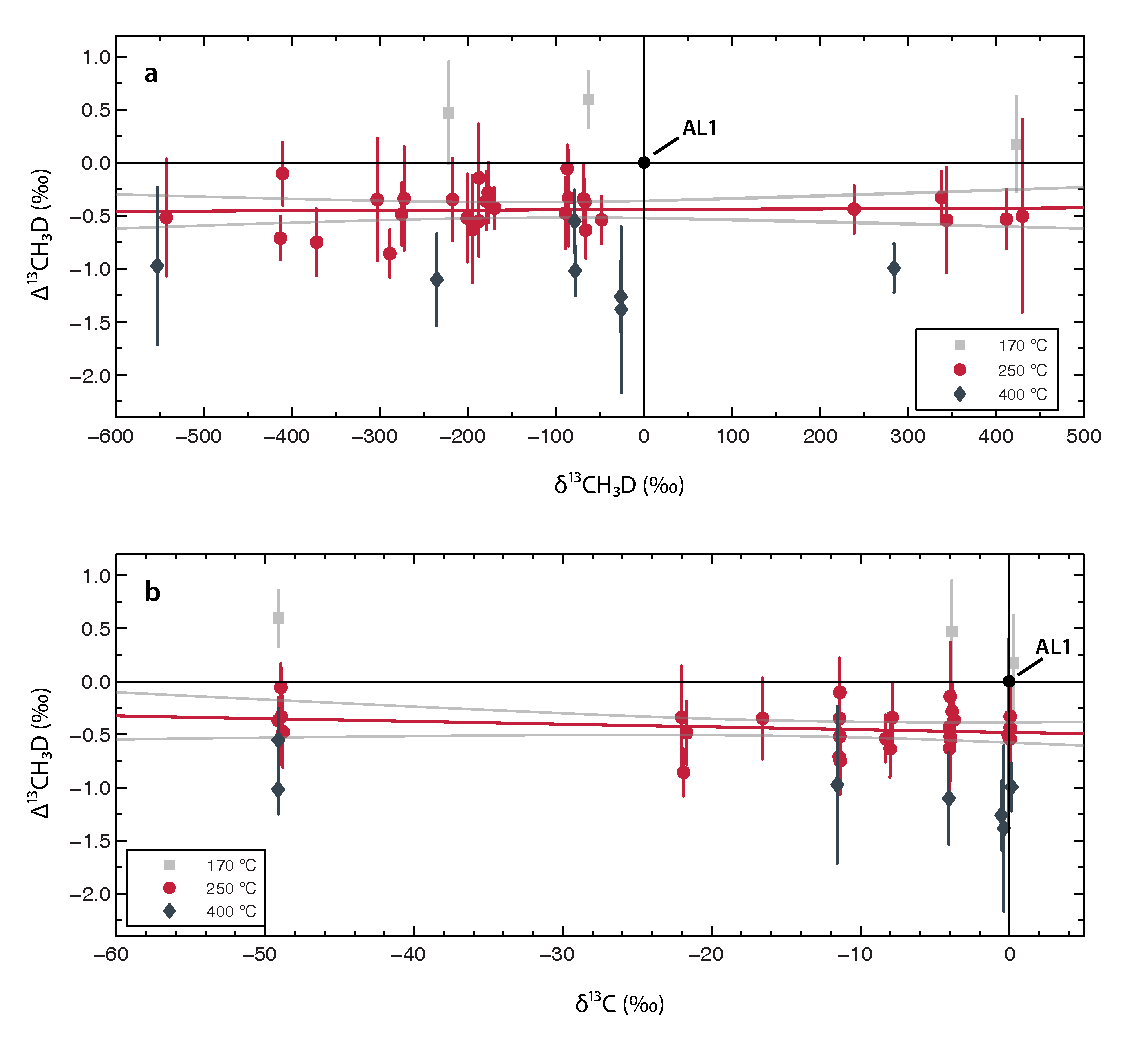
\includegraphics[width=0.85\linewidth]{figures/Fig2.S2}
	\caption[Demonstration of linearity in Δ\textsuperscript{13}CH\textsubscript{3}D over a range of bulk isotope ratios]{Demonstration of linearity in Δ\textsuperscript{13}CH\textsubscript{3}D over a range of bulk isotope ratios.  Shown are measurements of methane heated over catalyst at three
		temperatures (170, 250, 400~°C).  Solid red lines represent unweighted linear least squares
	regressions through gases equilibrated at 250~°C, and gray lines denote
	the 95\% confidence band. Error bars represent 95\% confidence intervals
	on multiple measurement cycles of a single analysis. Isotopic ratios are
	shown relative to our reference gas, AL1. Results indicate no
	significant correlation between
	Δ\textsuperscript{13}CH\textsubscript{3}D and (\textbf{A})
	δ\textsuperscript{13}CH\textsubscript{3}D over an 800‰ range (the
	variation in δ\textsuperscript{13}CH\textsubscript{3}D is driven mainly
	by differences in δD); and (\textbf{B}) δ\textsuperscript{13}C over a
	48‰ range.}
	\label{fig:2:S2}
\end{figure*}
